\documentclass[11pt]{llncs}

\def\makeitbig{%
\setlength{\textwidth}{15.9cm}%
\setlength{\oddsidemargin}{.01cm}%
\setlength{\evensidemargin}{.01cm}%
\setlength{\textheight}{21.5cm}%
\setlength{\topmargin}{-.25cm}%
\setlength{\headheight}{.7cm}%
\leftmargini 20pt     \leftmarginii 20pt%
\leftmarginiii 20pt   \leftmarginiv 20pt%
\leftmarginv 12pt     \leftmarginvi 12pt%
\pagestyle{myheadings}}%
\makeitbig

\usepackage{etex}
\usepackage{epsfig,tikz,amsmath,amsfonts,amssymb,verbatim,algorithm,algorithmic,program,rotating}
\usepackage[clock,weather,misc]{ifsym}
\usetikzlibrary{mindmap,trees,shadows}
\reserveinserts{28}

\usepackage{environ}
\makeatletter
\newsavebox{\measure@tikzpicture}
\NewEnviron{scaletikzpicturetowidth}[1]{%
  \def\tikz@width{#1}%
  \def\tikzscale{1}\begin{lrbox}{\measure@tikzpicture}%
  \BODY
  \end{lrbox}%
  \pgfmathparse{#1/\wd\measure@tikzpicture}%
  \edef\tikzscale{\pgfmathresult}%
  \BODY
}
\makeatother

\newcommand{\atk}{\begin{turn}{130}{\scriptsize \Lightning}\end{turn}}
\newcommand{\qm}{\raisebox{0.5ex}{\tiny ?}}
\newcommand{\tk}{\raisebox{1ex}{\atk}}
\newcommand{\ep}{\varepsilon}
\newcommand{\VV}[2]{\begin{tabular}{ll}
\tk&$\mathcal{V}_{#1}$\\
{\scriptsize \StopWatchEnd}& #2
\end{tabular}}
\newcommand{\PP}[1]{\tk $\mathcal{V}_{#1}$}
\newcommand{\LL}[2]{\mbox{\tk $\mathcal{V}_{#1}$,~{\scriptsize \StopWatchEnd} #2}}
\newcommand{\muk}{
\begin{tikzpicture}{\node[shape=circle,draw,inner sep=0.5pt, line width=0.3ex, fill=green, color=green, text=black] {{\tiny ?}};}\end{tikzpicture}}%
\newcommand{\blackbar}{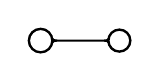
\begin{tikzpicture}[
  mindmap,
  every node/.style={concept, execute at begin node=\hskip0pt, font=\tiny},
  every concept/.style={minimum size=0.2cm, text width=0.2cm, fill=white, line width=0.2ex, text=black},
  text=white, grow cyclic,
  level 1/.append style={level distance=1cm,sibling angle=180}
]
\node {\raisebox{0.75ex}{}} child { node {}};
\end{tikzpicture}}
\newcommand{\bluebar}{\begin{tikzpicture}[
  mindmap,
  every node/.style={concept, execute at begin node=\hskip0pt, font=\tiny},
  every concept/.style={minimum size=0.2cm, text width=0.2cm, fill=white, line width=0.2ex, text=black},
  text=white, grow cyclic,
  level 1/.append style={level distance=1cm,sibling angle=180}
]
\node {\raisebox{0.75ex}{}} child[success=1] { node {}};
\end{tikzpicture}}
\newcommand{\redbar}{\begin{tikzpicture}[
  mindmap,
  every node/.style={concept, execute at begin node=\hskip0pt, font=\tiny},
  every concept/.style={minimum size=0.2cm, text width=0.2cm, fill=white, line width=0.2ex, text=black},
  text=white, grow cyclic,
  level 1/.append style={level distance=1cm,sibling angle=180}
]
\node {\raisebox{0.75ex}{}} child[failed=1] { node {}};
\end{tikzpicture}}
\newcommand{\ignore}[1]{}
\newcommand{\abs}[1]{\left|#1\right|}

\begin{document}



\title{Cascade {\sl Cryptanalysis} {\it Exemple}}

\author{Eric Brier\inst{1} \and Eric Freysinnet\inst{2} \and David Naccache\inst{3} \and Maxime Legrand\inst{3}  \and Thomas Magnard\inst{3} \and Marc Pasqualetto \inst{3} \and Nissim Zerbib\inst{3}}

\institute{%
Ingenico\\
1, rue Claude Chappe, {\sc bp 346}, {\sc f}-07503 Guilherand-Granges, France\\
\email{eric.brier@ingenico.com}
\and
LIP6, CNRS et Universit� Pierre et Marie Curie\\
4 place Jussieu - BC 169
{\sc f}-75252 Paris {\sc cedex 05}, France\\
\email{eric.freyssinet@botnets.fr}
\and
\'Ecole normale sup\'erieure\\
\'Equipe de cryptographie,
45 rue d'Ulm, {\sc f}-75230 Paris {\sc cedex 05}, France\\
\email{david.naccache@ens.fr, legrand.maxime@ens.fr, thomas.magnard@ens.fr,  marc.pasqualetto@ens.fr,  nissim.zerbib@ens.fr}
}

\maketitle

\begin{abstract}
...
\end{abstract}

\section{Introduction}




\makeatletter

\tikzoption{failed}{%
   \def\tikz@edge@to@parent@path{
     (\tikzparentnode)
     to[circle connection bar switch color=from (red) to (red)]
     (\tikzchildnode)}
   \def\tikz@concept@color{black}%
}

\tikzoption{success}{%
   \def\tikz@edge@to@parent@path{
     (\tikzparentnode)
     to[circle connection bar switch color=from (blue) to (blue)]
     (\tikzchildnode)}
   \def\tikz@concept@color{black}%
}

%%%%%%%%

\begin{figure}
\begin{center}
\begin{scaletikzpicturetowidth}{\textwidth}
\begin{tikzpicture}[scale=\tikzscale,
  mindmap,
  every node/.style={concept, execute at begin node=\hskip0pt, font=\small},
  every concept/.style={minimum size=0.4cm, text width=0.4cm, fill=white, line width=0.3ex, text=black},
  text=white, grow cyclic,
  level 1/.append style={level distance=0.2cm,sibling angle=180},
  level 2/.append style={level distance=0.1cm,sibling angle=90},
  level 3/.append style={level distance=0.1cm,sibling angle=45},
  level 4/.append style={level distance=0.1cm,sibling angle=45},
  level 5/.append style={level distance=0.065cm,sibling angle=0}
]

\node[dashed] {\raisebox{0.75ex}{$\bigtriangleup_1$}} % root
child[success=1] { node[minimum size=0.1cm, text width=0.1cm,font=\tiny, concept color=green, fill=green, line width=0ex] {\qm}
          child[success=1] { node {$\mathcal{V}_2$}
                child[success=1] { node[minimum size=0.1cm, text width=0.1cm,font=\tiny, concept color=green, fill=green, line width=0ex] {\qm}
                        child[success=1] { node {$\mathcal{V}_3$} child { node {$\mathcal{V}_4$}}}
                        child[success=1] { node {$\mathcal{V}_4$} child { node {$\mathcal{V}_3$}}}
                      }
                child[failed=1] { node[minimum size=0.1cm, text width=0.1cm,font=\tiny, concept color=green, fill=green, line width=0ex] {\qm}
                        child[failed=1] { node[failed=1] {$\mathcal{V}_3$} child { node {$\mathcal{V}_4$}}}
                        child[failed=1] { node {$\mathcal{V}_4$} child { node {$\mathcal{V}_3$}}}
                      }
                }
          child[success=1] { node {$\mathcal{V}_3$}
                child[success=1] { node[minimum size=0.1cm, text width=0.1cm,font=\tiny, concept color=green, fill=green, line width=0ex] {\qm}
                        child[success=1] { node {$\mathcal{V}_2$} child { node {$\mathcal{V}_4$}}}
                        child[success=1] { node {$\mathcal{V}_4$} child { node {$\mathcal{V}_2$}}}
                      }
                child[failed=1] { node[minimum size=0.1cm, text width=0.1cm,font=\tiny, concept color=green, fill=green, line width=0ex] {\qm}
                        child[failed=1] { node {$\mathcal{V}_2$} child { node {$\mathcal{V}_4$}}}
                        child[failed=1] { node {$\mathcal{V}_4$} child { node {$\mathcal{V}_2$}}}
                      }
                }
          child[success=1] { node {$\mathcal{V}_4$}
                child[success=1] { node[minimum size=0.1cm, text width=0.1cm,font=\tiny, concept color=green, fill=green, line width=0ex] {\qm}
                        child[success=1] { node {$\mathcal{V}_2$} child { node {$\mathcal{V}_3$}}}
                        child[success=1] { node {$\mathcal{V}_3$} child { node {$\mathcal{V}_2$}}}
                      }
                child[failed=1] { node[minimum size=0.1cm, text width=0.1cm,font=\tiny, concept color=green, fill=green, line width=0ex] {\qm}
                        child[failed=1] { node {$\mathcal{V}_2$} child { node {$\mathcal{V}_3$}}}
                        child[failed=1] { node {$\mathcal{V}_3$} child { node {$\mathcal{V}_2$}}}
                      }
                }}
child[failed=1] { node[minimum size=0.1cm, text width=0.1cm,font=\tiny, concept color=green, fill=green, line width=0ex] {\qm}
          child[failed=1] { node {$\mathcal{V}_2$}
                child[success=1] { node[minimum size=0.1cm, text width=0.1cm,font=\tiny, concept color=green, fill=green, line width=0ex] {\qm}
                        child[success=1] { node {$\mathcal{V}_3$} child { node {$\mathcal{V}_4$}}}
                        child[success=1] { node {$\mathcal{V}_4$} child { node {$\mathcal{V}_3$}}}
                      }
                child[failed=1] { node[minimum size=0.1cm, text width=0.1cm,font=\tiny, concept color=green, fill=green, line width=0ex] {\qm}
                        child[failed=1] { node[failed=1] {$\mathcal{V}_3$} child { node {$\mathcal{V}_4$}}}
                        child[failed=1] { node {$\mathcal{V}_4$} child { node {$\mathcal{V}_3$}}}
                      }
                }
          child[failed=1] { node {$\mathcal{V}_3$}
                child[success=1] { node[minimum size=0.1cm, text width=0.1cm,font=\tiny, concept color=green, fill=green, line width=0ex] {\qm}
                        child[success=1] { node {$\mathcal{V}_2$} child { node {$\mathcal{V}_4$}}}
                        child[success=1] { node {$\mathcal{V}_4$} child { node {$\mathcal{V}_2$}}}
                      }
                child[failed=1] { node[minimum size=0.1cm, text width=0.1cm,font=\tiny, concept color=green, fill=green, line width=0ex] {\qm}
                        child[failed=1] { node {$\mathcal{V}_2$} child { node {$\mathcal{V}_4$}}}
                        child[failed=1] { node {$\mathcal{V}_4$} child { node {$\mathcal{V}_2$}}}
                      }
                }
          child[failed=1] { node {$\mathcal{V}_4$}
                child[success=1] { node[minimum size=0.1cm, text width=0.1cm,font=\tiny, concept color=green, fill=green, line width=0ex] {\qm}
                        child[success=1] { node {$\mathcal{V}_2$} child { node {$\mathcal{V}_3$}}}
                        child[success=1] { node {$\mathcal{V}_3$} child { node {$\mathcal{V}_2$}}}
                      }
                child[failed=1] { node[minimum size=0.1cm, text width=0.1cm,font=\tiny, concept color=green, fill=green, line width=0ex] {\qm}
                        child[failed=1] { node {$\mathcal{V}_2$} child { node {$\mathcal{V}_3$}}}
                        child[failed=1] { node {$\mathcal{V}_3$} child { node {$\mathcal{V}_2$}}}
                      }
                }
      };
\end{tikzpicture}
\end{scaletikzpicturetowidth}
\end{center}
\caption{Finding an adaptive $P_{\mbox{\scriptsize {\sf opt}}}$ for $n=4$ (Assuming that it is known that the attack should start by $\mathcal{V}_1$).}
\label{dig1}
\end{figure}

Botnets are networks of infected end-hosts called bots that are under the control of a human operator commonly known as the botmaster (hereafter Alice). While botnets recruit vulnerable machines using methods also utilized by other classes of malware ({\sl e.g.}, remotely exploiting software vulnerabilities, social engineering, etc.), their defining characteristic is the use of command and control (C\&C) channels to connect bots to their botmasters. Bot owners are usually unaware that their computers were hijacked to forward transmissions ({\sl e.g.} spam or viruses) to other potential victims on the Internet.\smallskip

Computers hijacked into a botnet are often those whose owners fail to adequately protect. A bot is often created through an Internet port that has been left open and through which a malicious program can sneak in for future activation. At a certain time, Alice can unleash the effects of the botnet by sending a single command, possibly from an Internet Relay Channel (IRC) site.\smallskip

We model botnets in a very simple way: each target computer $\mathcal{V}_i$ is assimilated to a black-box having three attributes denoted $\epsilon_i,w_i,\pi_i$. $\mathcal{V}_i$ can be successfully attacked with probability $\epsilon_i$ by executing $w_i$ instructions. As in the Japanese go game (or the {\sl World War Z} movie), as soon as $\mathcal{V}_i$ is conquered, $\mathcal{V}_i$ can be used to attack other targets. The computational power provided by a conquered $\mathcal{V}_i$ is $\pi_i$ instructions per second. Alice's initial computational power is $A$\footnote{$A=1$ if the unit in which the $\pi_i$ are expressed is not instructions per second but "Alice-equivalents".}.\smallskip

This article attempts to clarify the following question:\smallskip

\begin{center}
\begin{tabular}{|l|}\hline
~~{\sl Given $n$ potential targets $\mathcal{V}_1,\ldots,\mathcal{V}_n$, how should Alice schedule her attacks to}~~\\
~~{\sl conquer all possible targets as quickly as possible?}~~\\\hline
\end{tabular}
\end{center}

Every attack plan $P$ has an expected completion time $\Delta(P)$.\smallskip

$P$ can be {\sl deterministic} or {\sl adaptive}. In a deterministic attack plan, Alice must define in advance the instant at which each $\mathcal{V}_i$ will be attacked. Attacks will be automatically launched as planned regardless successes or failures. An adaptive attacker has more freedom and progressively adapts her actions to observed successes or failures.\smallskip

In a deterministic {\sl sequential} plan, $P$ is a permutation of $\{1,\ldots,n\}$. In more general settings, plans may involve {\sl concurrency} ({\sl i.e.} distribute the available computational power between several simultaneous attacks) and {\sl pauses} ({\sl i.e.} halt an attack at a certain point in time and resume it later). This work does not deal with concurrency and pauses.\smallskip

To simplify diagrams, the pictographs \LL{i}{$t_i$} will mean {\sl "Alice attacks $\mathcal{V}_i$ and this attack requires $t_i$ time units"}. $\Gamma_n$ will denote the set of $n!$ permutations of $\{1,\ldots,n\}$.

As we will see, even this very simplified model requires involved analysis. Hence, real-life attacks that involve tens of other parameters would require much more complex heuristics.

\section{Deterministic Sequential Attacks}

In a {\sl deterministic sequential} plan, $P\in\Gamma_n$. Hence, Alice's goal is to find the $P_{\mbox{{\tiny op}}}$ that minimizes $\Delta_{\mbox{{\tiny det}}}(P)$.\smallskip

A glance at the small example $\Delta_{\mbox{{\tiny det}}}(\{1,2,3,4\})$ easily reveals the structure of $\Delta_{\mbox{{\tiny det}}}(P)$:

\tikzstyle{level 1}=[level distance=1cm, sibling distance=8cm]
\tikzstyle{level 2}=[level distance=3cm, sibling distance=4cm]
\tikzstyle{level 3}=[level distance=4.5cm, sibling distance=2.5cm]

\tikzstyle{bag} = [text width=7em, align=flush left] %text centered]
\tikzstyle{bag2} = [text width=7.5em, text centered]

\begin{tikzpicture}[->, grow=right, sloped]
\node[bag2] {\LL{1}{$\frac{w_1}{A}$}}
    child {
        node[bag2] {\LL{2}{$\frac{w_2}{A}$}}
 child {
        node[bag2] {\LL{3}{$\frac{w_3}{A}$}}
        child {
                node[bag] {\LL{4}{$\frac{w_4}{A}$}}
                edge from parent
                node[above] {failure}
                node[below] {$1-\epsilon_3$}
            }
            child {
                node[bag]{\LL{4}{$\frac{w_4}{A+\pi_3}$}}
                edge from parent
                node[above] {success}
                node[below]  {$\epsilon_3$}
            }
                edge from parent
                node[above] {failure}
                node[below]  {$1-\epsilon_2$}
             }
 child {
        node[bag2] {\LL{3}{$\frac{w_3}{A+\pi_2}$}}
        child {
                node[bag] {\LL{4}{$\frac{w_4}{A+\pi_2}$}}
                edge from parent
                node[above] {failure}
                node[below]  {$1-\epsilon_3$}
            }
            child {
                node[bag]{\LL{4}{$\frac{w_4}{A+\pi_2+\pi_3}$}}
                edge from parent
                node[above] {success}
                node[below]  {$\epsilon_3$}
            }
                edge from parent
                node[above] {success}
                node[below]  {$\epsilon_2$}
             }
            edge from parent
            node[above] {failure}
            node[below]  {$1-\epsilon_1$}
    }
    child {
        node[bag2] {\LL{2}{$\frac{w_2}{A+\pi_1}$}}
   child {
        node[bag2] {\LL{3}{$\frac{w_3}{A+\pi_1}$}}
        child {
                node[bag] {\LL{4}{$\frac{w_4}{A+\pi_1}$}}
                edge from parent
                node[above] {failure}
                node[below]  {$1-\epsilon_3$}
            }
            child {
                node[bag]{\LL{4}{$\frac{w_4}{A+\pi_1+\pi_3}$}}
                edge from parent
                node[above] {success}
                node[below]  {$\epsilon_3$}
            }
                edge from parent
                node[above] {failure}
                node[below]  {$1-\epsilon_2$}
             }
             child {
        node[bag2] {\LL{3}{$\frac{w_3}{A+\pi_1+\pi_2}$}}
        child {
                node[bag] {\LL{4}{$\frac{w_4}{A+\pi_1+\pi_2}$}}
                edge from parent
                node[above] {failure}
                node[below]  {$1-\epsilon_3$}
            }
            child {
                node[bag]{\LL{4}{$\frac{w_4}{A+\pi_1+\pi_2+\pi_3}$}}
                edge from parent
                node[above] {success}
                node[below]  {$\epsilon_3$}
            }
                edge from parent
                node[above] {success}
                node[below]  {$\epsilon_2$}
             }
        edge from parent
            node[above] {success}
            node[below]  {$\epsilon_1$}
    };
\end{tikzpicture}

and mathematically:

\begin{alignat}{4}
\Delta_{\mbox{{\tiny det}}}(\{1,2,3,4\})= &&\nonumber\\
\epsilon_1 \epsilon_2 \epsilon_3 &\left(\frac{w_1}A+\frac{w_2}{A+\pi_1}+\frac{w_3}{A+\pi_1+\pi_2}+\frac{w_4}{A+\pi_1+\pi_2+\pi_3}\right)&+\nonumber\\
\epsilon_1 \epsilon_2 (1-\epsilon_3) &\left(\frac{w_1}A+\frac{w_2}{A+\pi_1}+\frac{w_3}{A+\pi_1+\pi_2}+\frac{w_4}{A+\pi_1+\pi_2}\right)&+ \nonumber\\
\epsilon_1 (1-\epsilon_2) \epsilon_3 &\left(\frac{w_1}A+\frac{w_2}{A+\pi_1}+\frac{w_3}{A+\pi_1}+\frac{w_4}{A+\pi_1+\pi_3}\right)&+ \nonumber\\
\epsilon_1 (1-\epsilon_2) (1-\epsilon_3) &\left(\frac{w_1}A+\frac{w_2}{A+\pi_1}+\frac{w_3}{A+\pi_1}+\frac{w_4}{A+\pi_1}\right)&+ \nonumber\\
(1-\epsilon_1) \epsilon_2 \epsilon_3 &\left(\frac{w_1}A+\frac{w_2}A+\frac{w_3}{A+\pi_2}+\frac{w_4}{A+\pi_2+\pi_3}\right)&+ \nonumber\\
(1-\epsilon_1) \epsilon_2 (1-\epsilon_3) &\left(\frac{w_1}A+\frac{w_2}A+\frac{w_3}{A+\pi_2}+\frac{w_4}{A+\pi_2}\right)&+\nonumber\\
(1-\epsilon_1) (1-\epsilon_2) \epsilon_3 &\left(\frac{w_1}A+\frac{w_2}A+\frac{w_3}A+\frac{w_4}{A+\pi_3}\right)&+\nonumber\\
(1-\epsilon_1) (1-\epsilon_2) (1-\epsilon_3) &\left(\frac{w_1}A+\frac{w_2}A+\frac{w_3}A+\frac{w_4}A\right) &\nonumber
\end{alignat}

For instance, the term:

$$\epsilon_1 (1-\epsilon_2) \epsilon_3 \left(\frac{w_1}A+\frac{w_2}{A+\pi_1}+\frac{w_3}{A+\pi_1}+\frac{w_4}{A+\pi_1+\pi_3}\right)$$

expresses the fact that when the attack starts, Alice must attack $\mathcal{V}_1$ using her own computer (during $\frac{w_1}A$ time units). Because $\mathcal{V}_1$ falls into Alice's hands ($\epsilon_1$), the attack on $\mathcal{V}_2$ uses both Alice's own means $A$ and $\mathcal{V}_1$'s captured power $\pi_1$. $\frac{w_2}{A+\pi_1}$ time units are hence required to attack $\mathcal{V}_2$ but this attack fails ($1-\epsilon_2$). Hence $\mathcal{V}_3$ is attacked using $A+\pi_1$ only during $\frac{w_3}{A+\pi_1}$ time. $\mathcal{V}_3$ falls ($\epsilon_3$) and Alice's power grows further to $A+\pi_1+\pi_3$ which allows her to complete the (last) attack on $\mathcal{V}_4$ in $\frac{w_4}{A+\pi_1+\pi_3}$ time units. In other words, the formula enumerates all success/failure scenarios and sums their respective time expectations.\smallskip

For arbitrary $n$, $\Delta_{\mbox{{\tiny det}}}$ is given by the following formula where $k[j]$ denotes $j$-th bit of the integer $k$:

$$\Delta_{\mbox{{\tiny det}}}(P)=\sum_{k=0}^{2^{n-1}-1}\prod_{j=0}^{n-2} \epsilon_{P(j+1)}^{k[j]} (1-\epsilon_{P(j+1)})^{1-k[j]} \sum_{i=1}^n \frac{w_{P(i)}}{A+\sum\limits_{\ell=0}^{i-2} k[\ell] \pi_{P(\ell+1)}}$$

The evolution of $\Delta_{\mbox{{\tiny det}}}$ is irregular because $\Delta_{\mbox{{\tiny det}}}(P)$ does not depend on $\pi_{P(n)}$ and $\epsilon_{P(n)}$. Thus, swapping $\mathcal{V}_{P(n)}$ with some another $\mathcal{V}_{i\neq P(n)}$ replaces two formula parameters by new ones. This may cause radical variations in $\Delta$.%\footnote{A (somewhat artificial) remedy would be to rectify the model and assume that after the last attack Alice needs to amortize the captured computational power to perform some constant computational task $w'$. We do not use this alternative definition here.}

\subsection{Particular cases}
	\subsubsection{Fixed powers}
		Let's assume all $\pi_i$ are equal to $p$, then by sorting all computers according to $f(w,\varepsilon)=\frac{\varepsilon}{w}$ in decreasing order, we obtain the optimal solution. The complexity of this algorithm is obviously the complexity of an efficient sort, that is $O(n\log n)$.
		\begin{proof}
We will suppose that the list of computer is sorted in decreasing order .

Let $\sigma$ be a permutation different from identity.

let $i= \min(1 \leq j \leq n , \sigma (j) > \sigma (j+1))$ i exist because $\sigma$ is not identity.

Then let $\omega$ such as $\omega = \sigma \circ (i \;\; i+1)$ where $(i \;\; i+1)$ represent the permutation of $i$ and $i+1$

Let $T(\sigma)$ the average time of the attack in the order of $\sigma$ and $T(\omega)$ the time of the attack with $\omega$

The only difference between trees of $\sigma$ and $\omega$ are branches at depth $i$ and $i+1$
Then in all branches we have if A is the power at depth $i$ of this branch  ,$u= \sigma (i)$ and $v= \sigma (i+1)$:
$ T(\sigma) - T(\omega)=\frac{w_u}{A} +\epsilon_u( \frac{w_v}{A+1} +(1- \epsilon_u)(\frac{w_v}{A})- 
\frac{w_v}{A} +\epsilon_v( \frac{w_u}{A+1}) +(1- \epsilon_v)(\frac{w_u}{A} = (\frac{-1}{A(A+1)})(\epsilon_u w_v-\epsilon_v w_u
=w_uw_v(\frac{1}{A(A+1)})(\frac{\epsilon_{v}}{w_v}-\frac{\epsilon_u}{w_u})\geq 0$
because $v < u$

So any order exept the decreasing one can be enhanced .Finally The decreasing order is the best.

		\end{proof}
%Cela ne marche pas.	\subsubsection{All probabilities equal to 1}
%		If all the $\varepsilon_i$ are equal to $1$, then we are able to find the best solution in $O(n\log n)$, by a small modification of the merge sort. Given the power $A(t)$ at some step $t$ of the algorithm, we can compare two computers $x$ and $y$ by comparing $f(x,y) = f((w_x, p_x), (w_y, p_y)) = \frac{w_x}{A(t)} + \frac{w_y}{A(t) + p_y}$ and $f(y,x)$.
\subsection{Computational Strategies}

%Recurrenceformule
We begin with the following formula :
\[
	T(2n, r) = \frac{2n!}{n!^2}(T(n, r)+T(n, r+n))
\]
\[
	T(2n+1, r) = \frac{2(n+1)!}{(n+1)!n!}(T(n+1, r)+T(n, r+n+1))
\]
\[
	T(1, r) = 2^r
\]

We assume $\exists K > 0, \forall n \geqslant 16, \forall r \in \mathbb{N}, T(n, r) \leqslant K(2^{3n+r})$, thereby :
\[
	T(2n, r) \leqslant \frac{4^n}{\sqrt{n\pi}}K(2^{3n+r}+2^{3n+n+r})
\]
also
\[
	T(2n+1, r) \leqslant \frac{4^n}{\sqrt{n\pi}}K(2^{3(n+1)+r}+2^{3n+n+r+1})
\]
thus
\[
	T(2n, r) \leqslant \frac{2}{\sqrt{n\pi}}K2^{3(2n)+r} \leqslant K2^{3(2n)+r}
\]
\[
	T(2n+1, r) \leqslant \frac{4}{\sqrt{n\pi}}K2^{3(2n)+r} \leqslant K2^{3(2n)+r}
\]
Furthermore it remains true for $n \leqslant 15$, donc par récurrence sur n, on a bien
\[
	\boxed{ \exists K > 0, \forall n \in \mathbb{N}, \forall r \in \mathbb{N}, T(n, r) \leqslant K(2^{3n+r}) }
\]

We did not find polynomial-time algorithms for computing $P_{\mbox{{\tiny op}}}$. However, as we will immediately see, the problem's complexity is (at most) exponential and not factorial.\smallskip

We first note that the computation of $P_{\mbox{{\tiny op}}}$ can be accelerated (by a constant factor) using early aborts\footnote{{\sl e.g.} start by recording $\Delta_{\mbox{{\tiny det}}}(P_0)$ as a best score and begin computing $\Delta_{\mbox{{\tiny det}}}(P_1)$. As soon as the summation of terms in $\Delta_{\mbox{{\tiny det}}}(P_1)$ exceeds $\Delta_{\mbox{{\tiny det}}}(P_0)$ stop and try $P_2$ etc} and by smartly recycling for $P_{i+1}$ computations performed for computing $P_i$.\smallskip

Also, if $P=\{P(1),\ldots,P(n-1),P(n)\}$ and $P'=\{P(1),\ldots,P(n-2),P(n),P(n-1)\}$ we observe that the common prefix $\{P(1),\ldots,P(n-2)\}$ can serve for the computation of both $\Delta_{\mbox{{\tiny det}}}(P)$ and $\Delta_{\mbox{{\tiny det}}}(P')$. Pushing this observation further, we get a divide and conquer algorithm: \smallskip

Let $n=2k$ and let $P_{\mbox{{\tiny op}}}^{2k}$ be the optimal plan for attacking $\mathcal{V}_1,\ldots,\mathcal{V}_{2k}$. Given the (unordered) list $\mathcal{V}_{P_{\mbox{{\tiny op}}}^{2k}(1)},\ldots,\mathcal{V}_{P_{\mbox{{\tiny op}}}^{2k}(k)}$ we can compute the (ordered) prefix $\{P_{\mbox{{\tiny op}}}^{2k}(1),\ldots,P_{\mbox{{\tiny op}}}^{2k}(k)\}$ of $P_{\mbox{{\tiny op}}}^{2k}$ without examining $\mathcal{V}_{P_{\mbox{{\tiny op}}}^{2k}(k+1)},\ldots,\mathcal{V}_{P_{\mbox{{\tiny op}}}^{2k}(2k)}$, {\sl i.e.} $\Delta_{\mbox{{\tiny det}}}(P_{\mbox{{\tiny op}}}^{2k})$ can be computed by generating and solving all $\binom{2k}{k}$ sub-problem pairs of size $k$.\smallskip

In other words, if the cost of finding $P_{\mbox{{\tiny op}}}^{2k}$ is $f(n)$ then, denoting $n=2^a$:

$$f(n)= \binom{n}{n/2} \times (1+2^{n/2}) f(\frac{n}2)
= \frac{2^a n! f(1)}{\prod_{i=1}^{a-1}(2^i)!} \sim c_1 2^{2^{a+1} + c_2 a - \frac{a^2}4}=
O(2^{3 n + c_2 \log_2 n- \frac{\log_2^2 n}4})=O(2^{3n})$$

where: $$c_1=\frac{f(1)\pi^2}{e^2}\mbox{~~and~~}c_2=\frac{5-2\log_2 \pi}4$$


	\subsection{Heuristics}
		
		A simple heuristic is to order the computers by a function of $w$, $\pi$ and $\varepsilon$ and possibly $A$. For example one can easily intuit $f(w, \pi, \varepsilon) = \frac{\pi\varepsilon}{w}$ to be interesting. This function indeed yields good results for small instance, but one can do better.
		Let us consider one instance of the problem and two computers $(w_i,\pi_i,\varepsilon_i)$ and $(w_j,\pi_j,\varepsilon_j)$. We can decide easily if it is better to attack one computer before immediately attacking the other.
		\begin{align*}
			\Delta( \{ i, j, \cdots \}) - 	\Delta( \{ j, i, \cdots \}) &=  \frac{w_i}{A} + \varepsilon_i \frac{w_j}{A + \pi_i} + (1 - \varepsilon_i) \frac{w_j}{A} - \left ( \frac{w_j}{A} + \varepsilon_j \frac{w_i}{A + \pi_j} + (1 - \varepsilon_j ) \frac{w_i}{A} \right ) \\
										&=   \varepsilon_i w_j \left ( \frac{1}{A + \pi_i} -\frac{1}{A} \right ) - \varepsilon_j w_i \left ( \frac{1}{A + \pi_j} -\frac{1}{A} \right )\\ 
										&= - \varepsilon_i w_j  \frac{\pi_i}{A(A + \pi_i )} + \varepsilon_j w_i  \frac{\pi_j}{A(A + \pi_j )} 
		\end{align*}
		Thus it follows that : \[ \Delta( \{ i, j, \cdots \}) < \Delta( \{ j, i, \cdots \}) \Leftrightarrow \varepsilon_i w_j  \frac{\pi_i}{A + \pi_i} > \varepsilon_j w_i  \frac{\pi_j}{A + \pi_j} \Leftrightarrow \frac{\varepsilon_i \pi_i}{w_i(A + \pi_i)} >  \frac{\varepsilon_j \pi_j}{w_j(A + \pi_j)} \]
		We can now order the computers according to the values (in decreasing order) of the function $f(A,w,\pi, \varepsilon) =\frac{\varepsilon \pi}{w(A + \pi)}$. Of course after the first step, we no longer have a fixed power, although we could take the mean of the values of $f$ on different branches. However keeping the initial power gives good approximation with the complexity of a sort.
		This heuristics works well because we approximate a permutation of the computer which, albeit potentially suboptimal, is close to a permutation that is not improvable by any transposition of the form $(i\;\; i+1)$
		

		Actually it is possible to obtain a permutation of the computers that can't be improved by any transposition of the form  $(i\;\; i+1)$, at the price of an increased complexity of $O(2^n)$. This highlights the difficulty of the problem, as it is possible to find instances where such an algorithm is stuck in a suboptimal solution.
		
		A simple way to achieve an approximation of the last algorithm, which is polynomial in time, is to take the mean across sampled paths.
\section{An Experimental Observation}

Can a $P_{\mbox{{\tiny op}}}^{n+1}$ be constructed by inserting $\mathcal{V}_{n+1}$ into $P_{\mbox{{\tiny op}}}^n$? It appears that such is frequently the case. This section provides experimental statistics about the ratio of configurations for which the insertion of $\mathcal{V}_5$ and $\mathcal{V}_6$ into a 4-target solution is possible.

\begin{program}
\mbox{We performed the following experiment}
\PROC |Experiment|(B_\pi,B_w) \BODY
  \FOR A:=1 \TO 400 \DO
   r_A:=0\\
    \FOR t:=1 \TO 800 \DO
    \FOR i:=1 \TO 6 \DO
       |generate randomly|~0.01 \leq \epsilon_i\leq 1\\
       |generate randomly|~1 \leq \pi_i\leq B_\pi\\
       |generate randomly|~1 \leq w_i\leq B_w \\
    \OD\\
     |compute|~P_{\mbox{{\tiny op}}}(\mathcal{V}_1,\ldots,\mathcal{V}_6)
     |compute|~P_{\mbox{{\tiny op}}}(\mathcal{V}_1,\ldots,\mathcal{V}_4)
     \IF P_{\mbox{{\tiny op}}}(\mathcal{V}_1,\ldots,\mathcal{V}_6)~|can be obtained by inserting 5 and 6 into|~P_{\mbox{{\tiny op}}}(\mathcal{V}_1,\ldots,\mathcal{V}_4)\\
     \THEN r_A:=r_A+\frac1{800}\\
     \FI\\
     \OD\\
     \OD\\
\end{program}

It appears that for large $A$ the success ratio $r_A$ tends to one. This phenomenon is arguably related to the fact that sorting the computers according %We do not have an explanation of this observation. However, if true, this could yield a polynomial-time algorithm that outputs $P_{\mbox{{\tiny op}}}$ with high probability for large $A$ values.

\begin{figure}[!h]
\begin{center}
%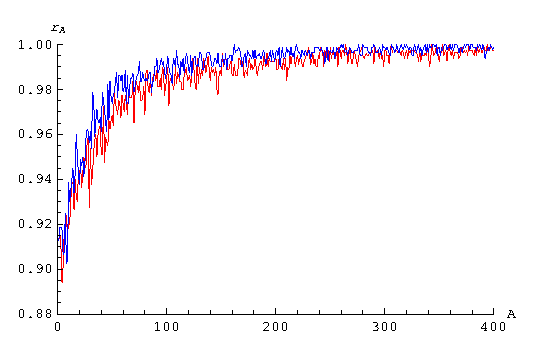
\includegraphics[width=10cm]{ordre.eps}
\end{center}
\caption{$\mbox{{\sf Experiment}}(100,100)$ (in red) and $\mbox{{\sf Experiment}}(50,200)$ (in blue). $r_A$ is the ratio of 6-target optimal plans obtainable by inserting 5 and 6 into their corresponding 4-target optimal plan.}
\label{fig}
\end{figure}

\section{Adaptive Attacks}

In an adaptive attack, Alice adapts future moves to successes and failures. To understand what an optimal adaptive attack is, assume that we already know (thanks to some oracle) that the best adaptive attack {\sl must} start by attacking $\mathcal{V}_1$. Before attacking $\mathcal{V}_1$ we face the two possible futures illustrated in Figures \ref{fut1} and \ref{fut2}:

\tikzstyle{level 1}=[level distance=4cm, sibling distance=4cm]
\tikzstyle{level 2}=[level distance=4cm, sibling distance=2cm]
\tikzstyle{bag2} = [text width=5em, align=flush left] %text centered]
\tikzstyle{bag3} = [text width=6em, text centered] %text centered]

\begin{figure}[!h]
\begin{center}
\begin{tikzpicture}[->, grow=right, sloped]
\node[bag2] {\LL{1}{$\frac{w_1}{A}$}}
    child {
        node[bag3] {\LL{2}{$\frac{w_2}{A}$}}
 child {
        node[bag2] {\LL{3}{$\frac{w_3}{A}$}}
                edge from parent
                node[above] {failure}
                node[below]  {$1-\epsilon_2$}
             }
 child {
        node[bag2] {\LL{3}{$\frac{w_3}{A+\pi_2}$}}
                edge from parent
                node[above] {success}
                node[below]  {$\epsilon_2$}
             }
            edge from parent
            node[above] {failure}
            node[below]  {$1-\epsilon_1$}
    }
    child {
        node[bag3] {\LL{2}{$\frac{w_2}{A+\pi_1}$}}
   child {
        node[bag2] {\LL{3}{$\frac{w_3}{A+\pi_1}$}}
                edge from parent
                node[above] {failure}
                node[below]  {$1-\epsilon_2$}
             }
             child {
        node[bag2] {\LL{3}{$\frac{w_3}{A+\pi_1+\pi_2}$}}
                edge from parent
                node[above] {success}
                node[below]  {$\epsilon_2$}
             }
        edge from parent
            node[above] {success}
            node[below]  {$\epsilon_1$}
    };
\end{tikzpicture}
\end{center}
\caption{First possible future after attacking $\mathcal{V}_1$: attack $\mathcal{V}_2$ first, $\mathcal{V}_3$ next.}
\label{fut1}
\end{figure}

\begin{figure}[!h]
\begin{center}
\begin{tikzpicture}[->, grow=right, sloped]
\node[bag2] {\LL{1}{$\frac{w_1}{A}$}}
    child {
        node[bag3] {\LL{3}{$\frac{w_3}{A}$}}
 child {
        node[bag2] {\LL{2}{$\frac{w_2}{A}$}}
                edge from parent
                node[above] {failure}
                node[below]  {$1-\epsilon_3$}
             }
 child {
        node[bag2] {\LL{2}{$\frac{w_2}{A+\pi_3}$}}
                edge from parent
                node[above] {success}
                node[below]  {$\epsilon_3$}
             }
            edge from parent
            node[above] {failure}
            node[below]  {$1-\epsilon_1$}
    }
    child {
        node[bag3] {\LL{3}{$\frac{w_3}{A+\pi_1}$}}
   child {
        node[bag2] {\LL{2}{$\frac{w_2}{A+\pi_1}$}}
                edge from parent
                node[above] {failure}
                node[below]  {$1-\epsilon_3$}
             }
             child {
        node[bag2] {\LL{2}{$\frac{w_2}{A+\pi_1+\pi_3}$}}
                edge from parent
                node[above] {success}
                node[below]  {$\epsilon_3$}
             }
        edge from parent
            node[above] {success}
            node[below]  {$\epsilon_1$}
    };
\end{tikzpicture}
\end{center}
\caption{Second possible future after attacking $\mathcal{V}_1$: attack $\mathcal{V}_3$ first, $\mathcal{V}_2$ next.}
\label{fut2}
\end{figure}

After attacking $\mathcal{V}_1$ the "dust settles" and Alice's information increases. Hence:

\begin{alignat*}{10}
&\Delta_{\mbox{\scriptsize {\sf ad}}}(\{1,\bullet,\bullet\})=\frac{w_1}{A}+ \\
\epsilon_1     & \min\bigg(\frac{w_2}{A+\pi_1}+\frac{\epsilon_2 w_3}{A+\pi_1+\pi_2}+\frac{(1-\epsilon_2) w_3}{A+\pi_1},\frac{w_3}{A+\pi_1}+\frac{\epsilon_3 w_2}{A+\pi_1+\pi_3}+\frac{(1-\epsilon_3) w_2}{A+\pi_1}\bigg)+\\
(1-\epsilon_1) & \min\bigg(\frac{w_2}{A}+\frac{\epsilon_2 w_3}{A+\pi_2}+\frac{(1-\epsilon_2) w_3}{A},\frac{w_3}{A}+\frac{\epsilon_3 w_2}{A+\pi_3}+\frac{(1-\epsilon_3) w_2}{A}\bigg)\\
\end{alignat*}

It appears that
\begin{gather*}
\frac{w_2}{A+\pi_1}+\frac{\epsilon_2 w_3}{A+\pi_1+\pi_2}+\frac{(1-\epsilon_2) w_3}{A+\pi_1}<\frac{w_3}{A+\pi_1}+\frac{\epsilon_3 w_2}{A+\pi_1+\pi_3}+\frac{(1-\epsilon_3) w_2}{A+\pi_1}\\
\Downarrow\\
\epsilon_2 w_3 \pi_2(A+\pi_1+\pi_3)>\epsilon_3 w_2 \pi_3(A+\pi_1+\pi_2)
\end{gather*}

and

\begin{gather*}
\frac{w_2}{A}+\frac{\epsilon_2 w_3}{A+\pi_2}+\frac{(1-\epsilon_2) w_3}{A}<\frac{w_3}{A}+\frac{\epsilon_3 w_2}{A+\pi_3}+\frac{(1-\epsilon_3) w_2}{A}\\
\Downarrow\\
\epsilon_2 w_3 \pi_2(A+\pi_3)>\epsilon_3 w_2 \pi_3(A+\pi_2)
\end{gather*}

Figures \ref{fut1} and \ref{fut2} can thus be merged into the unique plan shown in Figure \ref{comb}.

% Set the overall layout of the tree
\tikzstyle{level 1}=[level distance=1cm, sibling distance=8cm]
\tikzstyle{level 2}=[level distance=2cm, sibling distance=4cm]
\tikzstyle{level 3}=[level distance=4.5cm, sibling distance=2.5cm]

\tikzstyle{bag} = [text width=6em, text centered]
\tikzstyle{bag3} = [text width=20em, text centered]

\begin{figure}[!h]
\begin{center}
\begin{tikzpicture}[->, grow=right, sloped]
\node[bag] {\LL{1}{$\frac{w_1}{A}$}}
    child {
        node[bag3] {$\epsilon_2 w_3 \pi_2(A+\pi_3)>\epsilon_3 w_2 \pi_3(A+\pi_2)$}
 child {
        node[bag] {\LL{3}{$\frac{w_3}{A}$}}
        child {
                node[bag] {\LL{2}{$\frac{w_2}{A}$}}
                edge from parent
                node[above] {failure}
                node[below] {$1-\epsilon_3$}
            }
            child {
                node[bag]{\LL{2}{$\frac{w_2}{A+\pi_3}$}}
                edge from parent
                node[above] {success}
                node[below]  {$\epsilon_3$}
            }
                edge from parent
                node[above] {false}
             }
 child {
        node[bag] {\LL{2}{$\frac{w_2}{A}$}}
        child {
                node[bag] {\LL{3}{$\frac{w_3}{A}$}}
                edge from parent
                node[above] {failure}
                node[below]  {$1-\epsilon_2$}
            }
            child {
                node[bag]{\LL{3}{$\frac{w_3}{A+\pi_2}$}}
                edge from parent
                node[above] {success}
                node[below]  {$\epsilon_2$}
            }
                edge from parent
                node[above] {true}
             }
            edge from parent
            node[above] {failure}
            node[below]  {$1-\epsilon_1$}
    }
    child {
        node[bag3] {$\epsilon_2 w_3 \pi_2(A+\pi_1+\pi_3)>\epsilon_3 w_2 \pi_3(A+\pi_1+\pi_2)$}
   child {
        node[bag] {\LL{3}{$\frac{w_3}{A+\pi_1}$}}
        child {
                node[bag] {\LL{2}{$\frac{w_2}{A+\pi_1}$}}
                edge from parent
                node[above] {failure}
                node[below]  {$1-\epsilon_3$}
            }
            child {
                node[bag]{\LL{2}{$\frac{w_2}{A+\pi_1+\pi_3}$}}
                edge from parent
                node[above] {success}
                node[below]  {$\epsilon_3$}
            }
                edge from parent
                node[above] {false}
             }
             child {
        node[bag] {\LL{2}{$\frac{w_2}{A+\pi_1}$}}
        child {
                node[bag] {\LL{3}{$\frac{w_3}{A+\pi_1}$}}
                edge from parent
                node[above] {failure}
                node[below]  {$1-\epsilon_2$}
            }
            child {
                node[bag]{\LL{3}{$\frac{w_3}{A+\pi_1+\pi_2}$}}
                edge from parent
                node[above] {success}
                node[below]  {$\epsilon_2$}
            }
                edge from parent
                node[above] {true}
             }
        edge from parent
            node[above] {success}
            node[below]  {$\epsilon_1$}
    };
\end{tikzpicture}
\end{center}
\caption{Combined attack plan starting with $\mathcal{V}_1$.}
\label{comb}
\end{figure}

To find the best adaptive attack, Alice defines:

\begin{alignat*}{10}
&\Delta_{\mbox{\scriptsize {\sf ad}}}(\{x,\bullet,\bullet\})=\frac{w_x}{A}+ \\
(1-\epsilon_x) & \min\bigg(\frac{w_z}{A}+\frac{\epsilon_z w_y}{A+\pi_z}+\frac{(1-\epsilon_z) w_y}{A},\frac{w_y}{A}+\frac{\epsilon_y w_z}{A+\pi_y}+\frac{(1-\epsilon_y) w_z}{A}\bigg)\\
\epsilon_x     & \min\bigg(\frac{w_z}{A+\pi_x}+\frac{\epsilon_z w_y}{A+\pi_x+\pi_z}+\frac{(1-\epsilon_z) w_y}{A+\pi_x},\frac{w_y}{A+\pi_x}+\frac{\epsilon_y w_z}{A+\pi_x+\pi_y}+\frac{(1-\epsilon_y) w_z}{A+\pi_x}\bigg)\\
\end{alignat*}

and computes:

$$
\Delta_{\mbox{\scriptsize {\sf ad}}}(P_{\mbox{\scriptsize {\sf opt}}})
= \min_{\{x,y,z\}\in\Gamma_n}(\Delta_{\mbox{\scriptsize {\sf ad}}}(x,\bullet,\bullet))$$

Intuition suggests that an adaptive plan (allowing Alice more freedom of action) would yield better results than a deterministic one. Such is indeed the case, as shown in the following example\footnote{$\mathcal{V}_i=\{\pi_i,w_i,\epsilon_i\}$} where $A=7$, $n=3$ and $\mathcal{V}_1=\{2,1,0.3\}$, $\mathcal{V}_2=\{10,5,0.2\}$, $\mathcal{V}_3=\{1,2,0.4\}$ and:\smallskip

\begin{center}
\begin{tabular}{|l|c|c|c|c|c|c|}\hline
~~permutation $\rightarrow$~~&~$\{1,2,3\}$~&~$\{1,3,2\}$~&~$\{2,1,3\}$~&~$\{2,3,1\}$~&~$\{3,1,2\}$~&~$\{3,2,1\}$~\\\hline
~~$\Delta_{\mbox{\scriptsize {\sf det}}}$&  1.04564 &  1.04452 &   1.07646 & 1.08646  & 1.05643  & 1.08436 \\\hline
\end{tabular}
\end{center}

For $n=3$ adaptive attacks are not characterized by a permutation but by the $\mathcal{V}_i$ attacked first. It appears that:

\begin{alignat*}{10}
\Delta_{\mbox{\scriptsize {\sf det}}}(2,1,3)&=&\Delta_{\mbox{\scriptsize {\sf ad}}}(2,\bullet,\bullet)&=1.07646\\
\Delta_{\mbox{\scriptsize {\sf det}}}(3,1,2)&=&\Delta_{\mbox{\scriptsize {\sf ad}}}(3,\bullet,\bullet)&=1.05643\\
\mbox{but:}                                 & &\Delta_{\mbox{\scriptsize {\sf ad}}}(1,\bullet,\bullet)&=1.04417<\min_{\{x,y,z\}\in\Gamma_3}(\Delta_{\mbox{\scriptsize {\sf det}}}(x,y,z))=\Delta_{\mbox{\scriptsize {\sf det}}}(1,3,2)=1.04452\\
\end{alignat*}
\smallskip

\begin{alignat*}{10}
\mbox{Here:~~}\Delta_{\mbox{\scriptsize {\sf ad}}}(1,\bullet,\bullet)=\frac{w_1}A+(1-\epsilon_1) &\left(\frac{(1-\epsilon_3) w_2}A+\frac{\epsilon_3 w_2}{A+\pi_3}+\frac{w_3}{A}\right)+\\
            \epsilon_1 & \left(\frac{w_2}{A+\pi_1}+\frac{(1-\epsilon_2) w_3}{A+\pi_1}+\frac{\epsilon_2 w_3}{A+\pi_1+\pi_2}\right)=1.04417\\
\end{alignat*}

\tikzstyle{level 1}=[level distance=4cm, sibling distance=4cm]
\tikzstyle{level 2}=[level distance=4cm, sibling distance=2cm]
\tikzstyle{bag2} = [text width=5em, align=flush left] %text centered]
\tikzstyle{bag3} = [text width=6em, text centered] %text centered]

\begin{figure}[!h]
\begin{center}
\begin{tikzpicture}[->, grow=right, sloped]
\node[bag2] {\LL{1}{$\frac{1}{7}$}}
    child {
        node[bag3] {\LL{3}{$\frac{2}{7}$}}
 child {
        node[bag2] {\LL{2}{$\frac{5}{7}$}}
                edge from parent
                node[above] {failure}
                node[below]  {$1-0.4=0.6$}
             }
 child {
        node[bag2] {\LL{2}{$\frac{5}{7+1}=\frac58$}}
                edge from parent
                node[above] {success}
                node[below]  {$0.4$}
             }
            edge from parent
            node[above] {failure}
            node[below]  {$1-0.3=0.7$}
    }
    child {
        node[bag3] {\LL{2}{$\frac{5}{7+2}=\frac59$}}
   child {
        node[bag2] {\LL{3}{$\frac{2}{7+2}=\frac29$}}
                edge from parent
                node[above] {failure}
                node[below]  {$1-0.2=0.8$}
             }
             child {
        node[bag2] {\LL{3}{$\frac{2}{7+2+10}=\frac2{19}$}}
                edge from parent
                node[above] {success}
                node[below]  {$0.2$}
             }
        edge from parent
            node[above] {success}
            node[below]  {$0.3$}
    };
\end{tikzpicture}
\end{center}
\caption{The $1,\bullet,\bullet$ scenario (note that the order of attacks in the branches is reversed).}
\label{fut1}
\end{figure}



We have
\begin{align}
	\frac{\ep_2\pi_2}{w_2}(A+\pi_1+\pi_3) &> \frac{\ep_3\pi_3}{w_3}(A+\pi_1+\pi_2)\\
	\frac{\ep_2\pi_2}{w_2}(A+\pi_3) &< \frac{\ep_3\pi_3}{w_3}(A+\pi_2)
\end{align}
It follows that : 
\begin{align*}
	-\frac{\ep_2\pi_2}{w_2}(A+\pi_3) &> -\frac{\ep_3\pi_3}{w_3}(A+\pi_2)\\
	\frac{\ep_2\pi_2}{w_2}\pi_1 &> \frac{\ep_3\pi_3}{w_3}\pi_1\\
	\frac{\ep_2\pi_2}{w_2} &> \frac{\ep_3\pi_3}{w_3}\\
	-A\frac{\ep_2\pi_2}{w_2} &< -A\frac{\ep_3\pi_3}{w_3}\\
	\frac{\ep_2\pi_2}{w_2}\pi_3 &< \frac{\ep_3\pi_3}{w_3}\pi_2
\end{align*}
Finally :
\begin{align}
	\frac{\ep_2}{w_2} &> \frac{\ep_3}{w_3}\\
	\frac{\ep_2\pi_2}{w_2} &< \frac{\ep_3\pi_3}{w_3}
\end{align}
We can sum up :
\begin{align*}
	\frac{\ep_2\pi_2}{w_2\pi_3} >  \frac{\ep_3}{w_3} > \frac{\ep_2}{w_2}
\end{align*}

There is no dependency on $\pi_1$ because when only two computers are left, the current power 

The general algorithm is illustrated in Figures \ref{star} and \ref{dig1}. Assume again that we know (thanks to some oracle) that an adaptive attack for $n=4$ should start by $\mathcal{V}_1$. Figure \ref{dig1} shows the 4 possible attack plans starting by an attack on $\mathcal{V}_1$.\smallskip

To compute a time expectation of a branch, consider the chain of red and blue cells leading to the black leaf. The chain defines the computation power available for attacking the black leaf and hence the time taken to do so. Work the way up until a \muk\ is met. Then prune all branches except the one whose time is minimal and proceed further up. This will yield a decision tree representing the optimal adaptive moves.\smallskip

Now, because we are not given an oracle ({\sl i.e.} the optimal attack may begin by some $\mathcal{V}_i\neq\mathcal{V}_1$) the process must be repeated for all possible first targets as shown in Figure \ref{star}.\smallskip

The algorithm examines $2^n n!$ attack chains and prunes them to get the $2^n$ "recipe" describing how to best proceed adaptively.\smallskip

Here are the frequencies of different timings:

\begin{center}
{\small
\begin{tabular}{c|c}\hline
2 & \{4,1\}, \{2,2\}\\\hline
3 & \{12,1\}, \{2,12\}, \{4,3\}\\\hline
4 &\{48,1\}, \{4,36\}, \{2,72\}, \{12,4\}\\\hline
5 &\{240,1\}, \{12,60\}, \{8,30\}, \{4,300\}, \{2,600\}, \{48,5\}\\\hline
6 &\{1440,1\}, \{48,90\}, \{24,120\}, \{12,600\}, \{4,3600\}, \{8,360\}, \{2,5760\}, \{240,6\}\\\hline
7 &\{10080,1\}, \{240,126\}, \{96,210\}, \{48,1050\}, \{72,140\}, \{12,8400\}, \{24,1680\}, \{8,7560\}, \{4,45360\}, \{2,65520\}, \{1440,7\}\\\hline
\end{tabular}}
\end{center}

We could heuristically identify some of these entries as:

$$\{2 i!, 1\},~\{2, i! \phi(i)\},\{2(i-1)!,i\},\{2(i-2)!, 3i(i-1)\}$$

\begin{figure}
\begin{center}
\begin{tabular}{cc}
\begin{scaletikzpicturetowidth}{\textwidth}
\begin{tikzpicture}[scale=\tikzscale,
  mindmap,
  every node/.style={concept, execute at begin node=\hskip0pt, font=\small},
  every concept/.style={minimum size=0.4cm, text width=0.4cm, concept color=black, fill=white, line width=0.3ex, text=black},
  text=white, grow cyclic,
  level 1/.append style={level distance=0.05cm,sibling angle=180},
  level 2/.append style={level distance=0.05cm,sibling angle=45},
  level 3/.append style={level distance=0.05cm,sibling angle=0},
  level 4/.append style={level distance=0.05cm,sibling angle=0},
]

\node[minimum size=0.6cm, text width=0.6cm,font=\tiny, concept color=black, fill=white, line width=0ex, rectangle, rounded corners] {\raisebox{0.5ex}{\tiny start}}
child[success=1] { node[minimum size=0.1cm, text width=0.1cm,font=\tiny, concept color=green, fill=green, line width=0ex] {\qm}
          child[success=1] { node {4} child[dashed] { node[dashed] {\raisebox{0.75ex}{$\bigtriangleup_4$}}}}
          child[success=1] { node {3} child[dashed] { node[dashed] {\raisebox{0.75ex}{$\bigtriangleup_3$}}}}
          child[success=1] { node {2} child[dashed] { node[dashed] {\raisebox{0.75ex}{$\bigtriangleup_2$}}}}
          child[success=1] { node {1} child[dashed] { node[dashed] {\raisebox{0.75ex}{$\bigtriangleup_1$}}}}
    }
child[failed=1] { node[minimum size=0.1cm, text width=0.1cm,font=\tiny, concept color=green, fill=green, line width=0ex] {\qm}
          child[failed=1] { node {4} child[dashed] { node[dashed] {\raisebox{0.75ex}{$\bigtriangleup_4$}}}}
          child[failed=1] { node {3} child[dashed] { node[dashed] {\raisebox{0.75ex}{$\bigtriangleup_3$}}}}
          child[failed=1] { node {2} child[dashed] { node[dashed] {\raisebox{0.75ex}{$\bigtriangleup_2$}}}}
          child[failed=1] { node {1} child[dashed] { node[dashed] {\raisebox{0.75ex}{$\bigtriangleup_1$}}}}
          };
\end{tikzpicture}
\end{scaletikzpicturetowidth}&\raisebox{21ex}{
{\small
\begin{tabular}{|cll|}\hline
\raisebox{-0.6ex}{\bluebar}&~:&~the attack succeeded\\[-0.01cm]
\raisebox{-0.6ex}{\redbar}   &~:&~the attack failed\\[-0.01cm]
\raisebox{-0.6ex}{\blackbar} &~:&~last attack in branch (consider both success and failure)~\\[-0.01cm]
\raisebox{-0.6ex}{\muk}      &~:&~select the branch corresponding to the shortest time\\[-0.01cm]
$\bigtriangleup_i \mbox{~for~}i\neq 1$&~:&~$\bigtriangleup_1$ as in Figure \ref{dig1} where symbols $i$ and $1$ are swapped~\\[-0.01cm]\hline
\end{tabular}}}
\end{tabular}
\end{center}
\caption{Finding an adaptive $P_{\mbox{\scriptsize {\sf opt}}}$ for $n=4$ (start of process).}
\label{star}
\end{figure}

\begin{thebibliography}{30}

\bibitem{bot} http://searchsecurity.techtarget.com/definition/botnet

\bibitem{bot2} M. Abu Rajab, J. Zarfoss, F. Monrose, A. Terzis, A multifaceted approach to understanding the botnet phenomenon, in Proceedings of the 6th ACM SIGCOMM conference on Internet measurement (IMC �06)

\end{thebibliography}

\end{document}
